\documentclass[11pt,a4paper]{article}

\usepackage[margin=2.2cm]{geometry}
\usepackage{graphicx}
\usepackage{booktabs}
\usepackage{amsmath}
\usepackage{float}
\usepackage{caption}
\usepackage{subcaption}
\usepackage{multirow}
\usepackage[table]{xcolor}
\usepackage[hidelinks]{hyperref}
\usepackage{enumitem}

% Images live in results/ relative to this .tex file
\graphicspath{{results/}{./}}

\captionsetup{font=small,labelfont=bf}
\setlist{itemsep=2pt,topsep=4pt}

\title{\vspace{-1.5cm}\textbf{Assignment 2 --- Interpolation-Based Super-Resolution}}
\author{Om Kumar Gupta \\ B.Tech, Electronics and Communication Engineering \\ IIIT Delhi}
\date{\today}

\begin{document}
\maketitle

%==========================================================
\section{Objective}

The aim of this study is to evaluate classical interpolation-based super-resolution.
Four $512 \times 512$ grayscale images are downsampled to $64\times64$, $128\times128$ and
$256\times256$, then super-resolved back to $512\times512$ using interpolation kernels of
increasing order. Reconstruction quality is measured against the original image using PSNR
and SSIM, and the computational cost of each method is measured. The enlargement factors
under study are listed in Table~\ref{tab:settings}.

\begin{table}[H]
\centering
\caption{Super-resolution settings.}
\label{tab:settings}
\begin{tabular}{ccc}
\toprule
Input size & Output size & Enlargement factor \\
\midrule
$64\times64$   & $512\times512$ & $8\times$ \\
$128\times128$ & $512\times512$ & $4\times$ \\
$256\times256$ & $512\times512$ & $2\times$ \\
\bottomrule
\end{tabular}
\end{table}

%==========================================================
\section{Dataset}

Four images were taken from the Miscellaneous volume of the USC-SIPI image database
(\url{https://sipi.usc.edu/database/database.php?volume=misc}). They were selected to span
distinct content types --- dense texture, hard geometric edges, large smooth regions, and a
mixture --- so that the dependence of the results on image content could be examined.

\begin{table}[H]
\centering
\caption{Selected images. All were converted to 8-bit grayscale at $512\times512$ before
any processing.}
\label{tab:dataset}
\begin{tabular}{llll}
\toprule
SIPI id & Name & Native format & Content character \\
\midrule
4.2.03 & Mandrill / Baboon  & 24\,bpp colour & Dense high-frequency fur texture \\
4.2.05 & Airplane (F-16)    & 24\,bpp colour & Strong clean edges, flat sky \\
4.2.07 & Peppers            & 24\,bpp colour & Large smooth shaded regions \\
5.2.10 & Stream and bridge  & 8\,bpp gray    & Mixed texture and structure \\
\bottomrule
\end{tabular}
\end{table}

\begin{figure}[H]
\centering
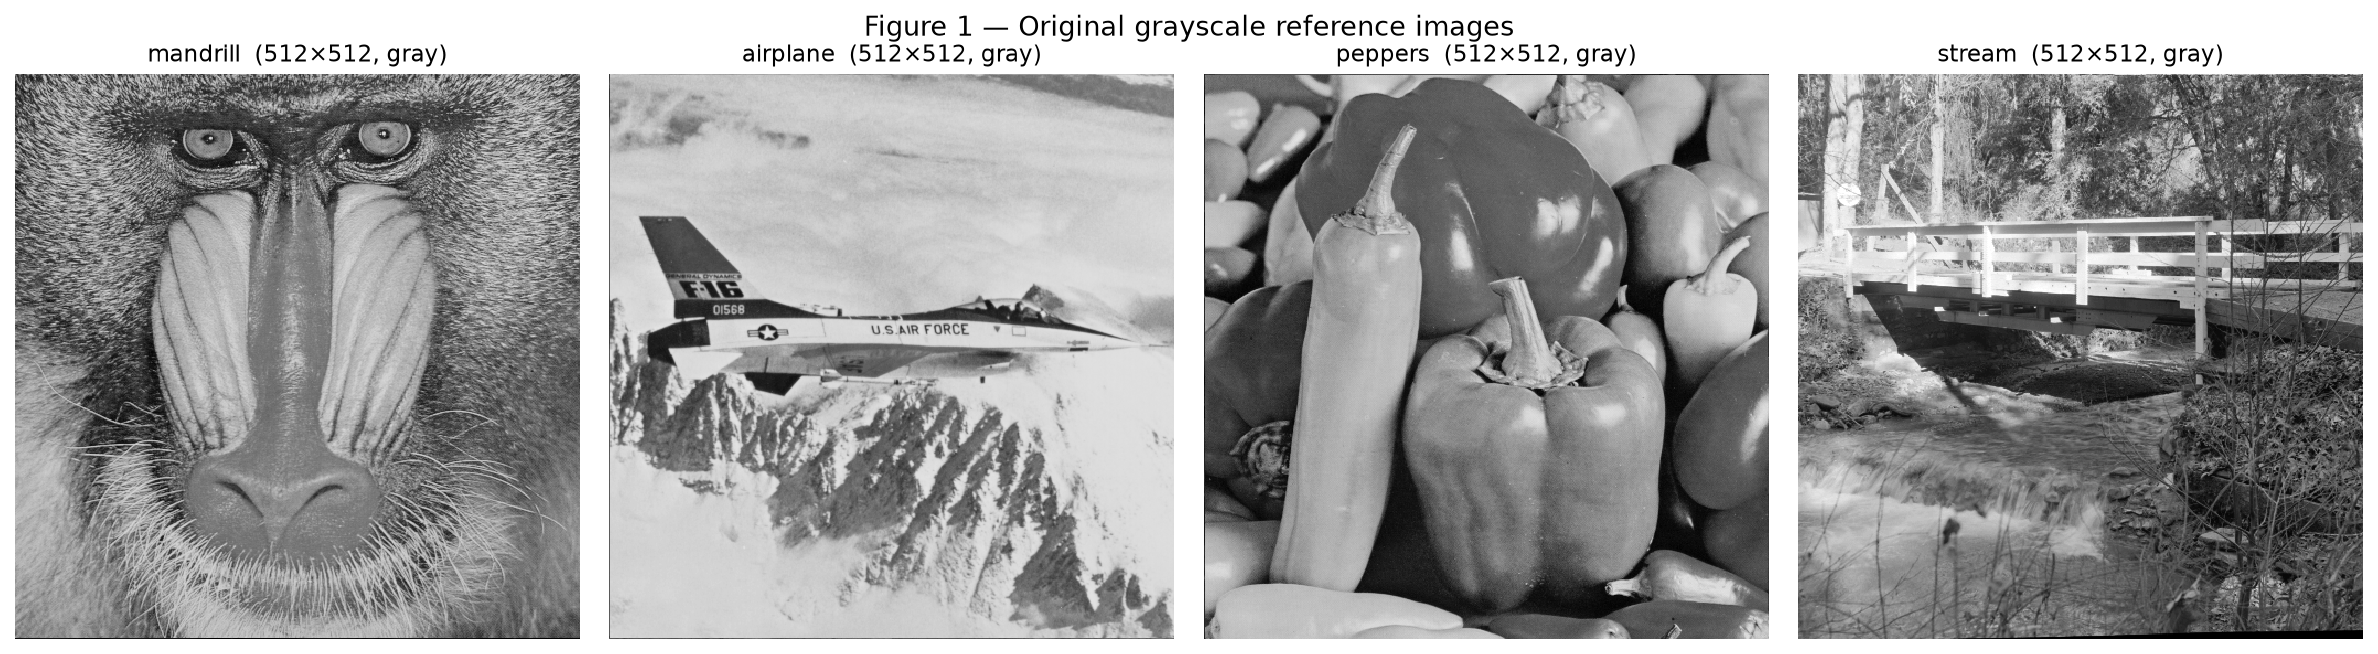
\includegraphics[width=\textwidth]{figures_fig1_originals.png}
\caption{The four original grayscale reference images ($512\times512$, 8\,bpp). These serve
as the ground truth for all PSNR and SSIM computations.}
\label{fig:originals}
\end{figure}

%==========================================================
\section{Methodology}

\subsection{Pipeline}

The processing order is fixed for all images:

\begin{enumerate}[label=\arabic*.]
  \item \textbf{Grayscale conversion.} Colour images are converted using ITU-R BT.601 luma
        weights. Images already stored as 8\,bpp monochrome are passed through unchanged.
        Conversion is performed \emph{before} downsampling so that all four images follow an
        identical path.
  \item \textbf{Downsampling.} The $512\times512$ grayscale reference is reduced to
        $256\times256$, $128\times128$ and $64\times64$ using area averaging
        (\texttt{cv2.INTER\_AREA}), i.e.\ a low-pass filter followed by decimation. The same
        function and the same flag are used for every image and every size throughout the
        study.
  \item \textbf{Super-resolution.} Each low-resolution image is interpolated back to
        $512\times512$.
  \item \textbf{Evaluation.} PSNR and SSIM are computed between each super-resolved output
        and the original $512\times512$ grayscale image, never against the low-resolution
        input.
\end{enumerate}

Area averaging was chosen over plain decimation deliberately. Plain decimation would alias
high-frequency content --- most severely on the mandrill --- before any interpolation took
place, which would corrupt every subsequent metric and make the comparison between methods
meaningless. Since $512/64$, $512/128$ and $512/256$ are exact powers of two, no fractional
pixel alignment arises at either stage.

\subsection{Interpolation methods}

Six methods were implemented, covering the orders named in the task plus a windowed-sinc
kernel for comparison.

\begin{table}[H]
\centering
\caption{Interpolation methods evaluated.}
\label{tab:methods}
\begin{tabular}{llll}
\toprule
Order & Method & Implementation & Kernel character \\
\midrule
0th & Nearest neighbour & scikit-image, \texttt{order=0} & Piecewise constant \\
1st & Bilinear          & scikit-image, \texttt{order=1} & Piecewise linear \\
2nd & Biquadratic       & scikit-image, \texttt{order=2} & Quadratic B-spline \\
3rd & Bicubic           & scikit-image, \texttt{order=3} & Cubic B-spline \\
5th & Biquintic         & scikit-image, \texttt{order=5} & Quintic B-spline \\
--- & Lanczos-4         & OpenCV, \texttt{INTER\_LANCZOS4} & Windowed sinc \\
\bottomrule
\end{tabular}
\end{table}

Orders 0--5 are all drawn from a single library so that the runtime column compares like with
like. OpenCV provides no second-, fourth- or fifth-order resize, so the spline family could
not be sourced from it; conversely scikit-image provides no Lanczos resize. The Lanczos-4
timing must therefore be read as a separate note rather than as a directly comparable
measurement --- this is discussed in Section~\ref{sec:runtime}.

Anti-aliasing is disabled for all upsampling operations, as it is a downsampling-only
concern. Kernels of order $\ge 2$ have negative lobes and can produce values outside
$[0,255]$ near strong edges; all outputs are clipped to $[0,255]$ and cast to \texttt{uint8}
before metrics are computed. Orders 0 and 1 have non-negative kernels and cannot overshoot by
construction.

\subsection{Measurement protocol}

PSNR and SSIM are computed on the full $512\times512$ frame with \texttt{data\_range=255},
using \texttt{skimage.metrics}. Runtime covers the interpolation call only --- no file I/O,
no metric computation, no plotting. Each configuration is executed once as a warm-up and then
timed over 10 further runs using \texttt{time.perf\_counter()}; the reported value is the
mean in milliseconds.

The full experiment is $4 \text{ images} \times 3 \text{ factors} \times 6 \text{ methods}
= 72$ super-resolved images and 72 measurement rows.

%==========================================================
\section{Results}

\subsection{Downsampled inputs}

\begin{figure}[H]
\centering
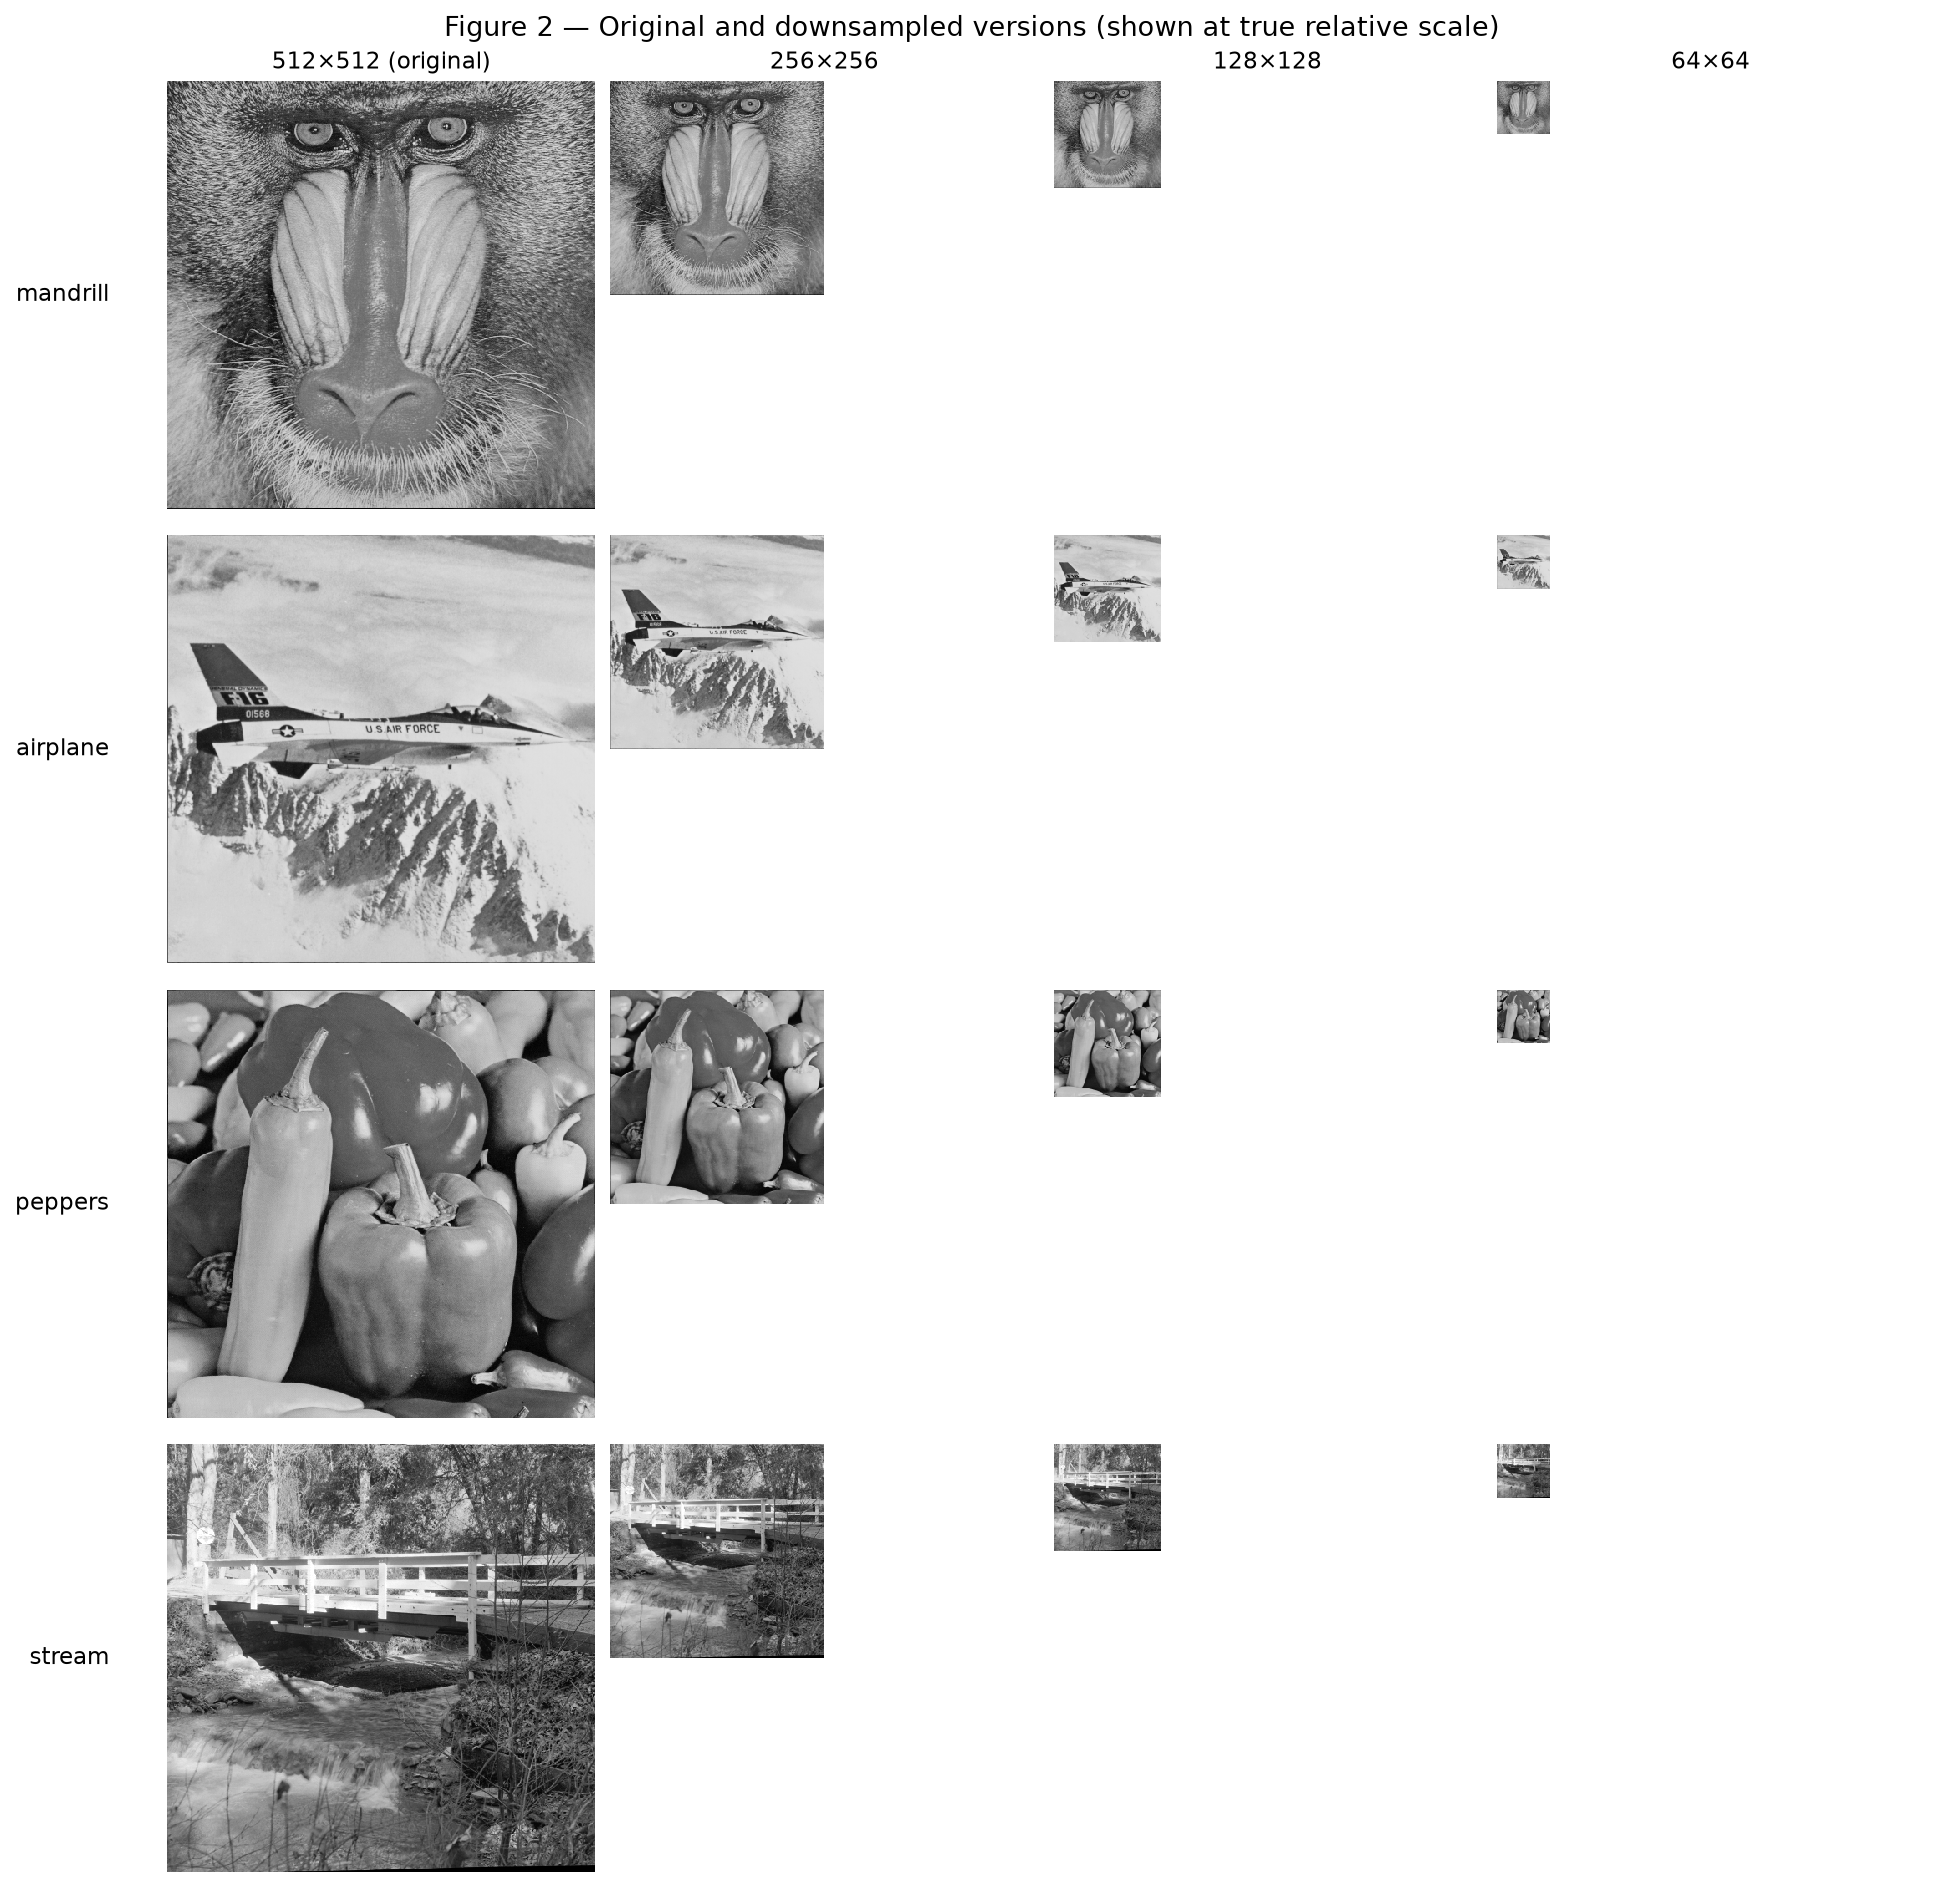
\includegraphics[width=\textwidth]{figures_fig2_downsampled.png}
\caption{Original and downsampled versions of each image, displayed at true relative scale.
The loss of fur texture in the $64\times64$ mandrill is total; no interpolation method can
recover it.}
\label{fig:downsampled}
\end{figure}

\subsection{Super-resolved outputs}

\begin{figure}[H]
\centering
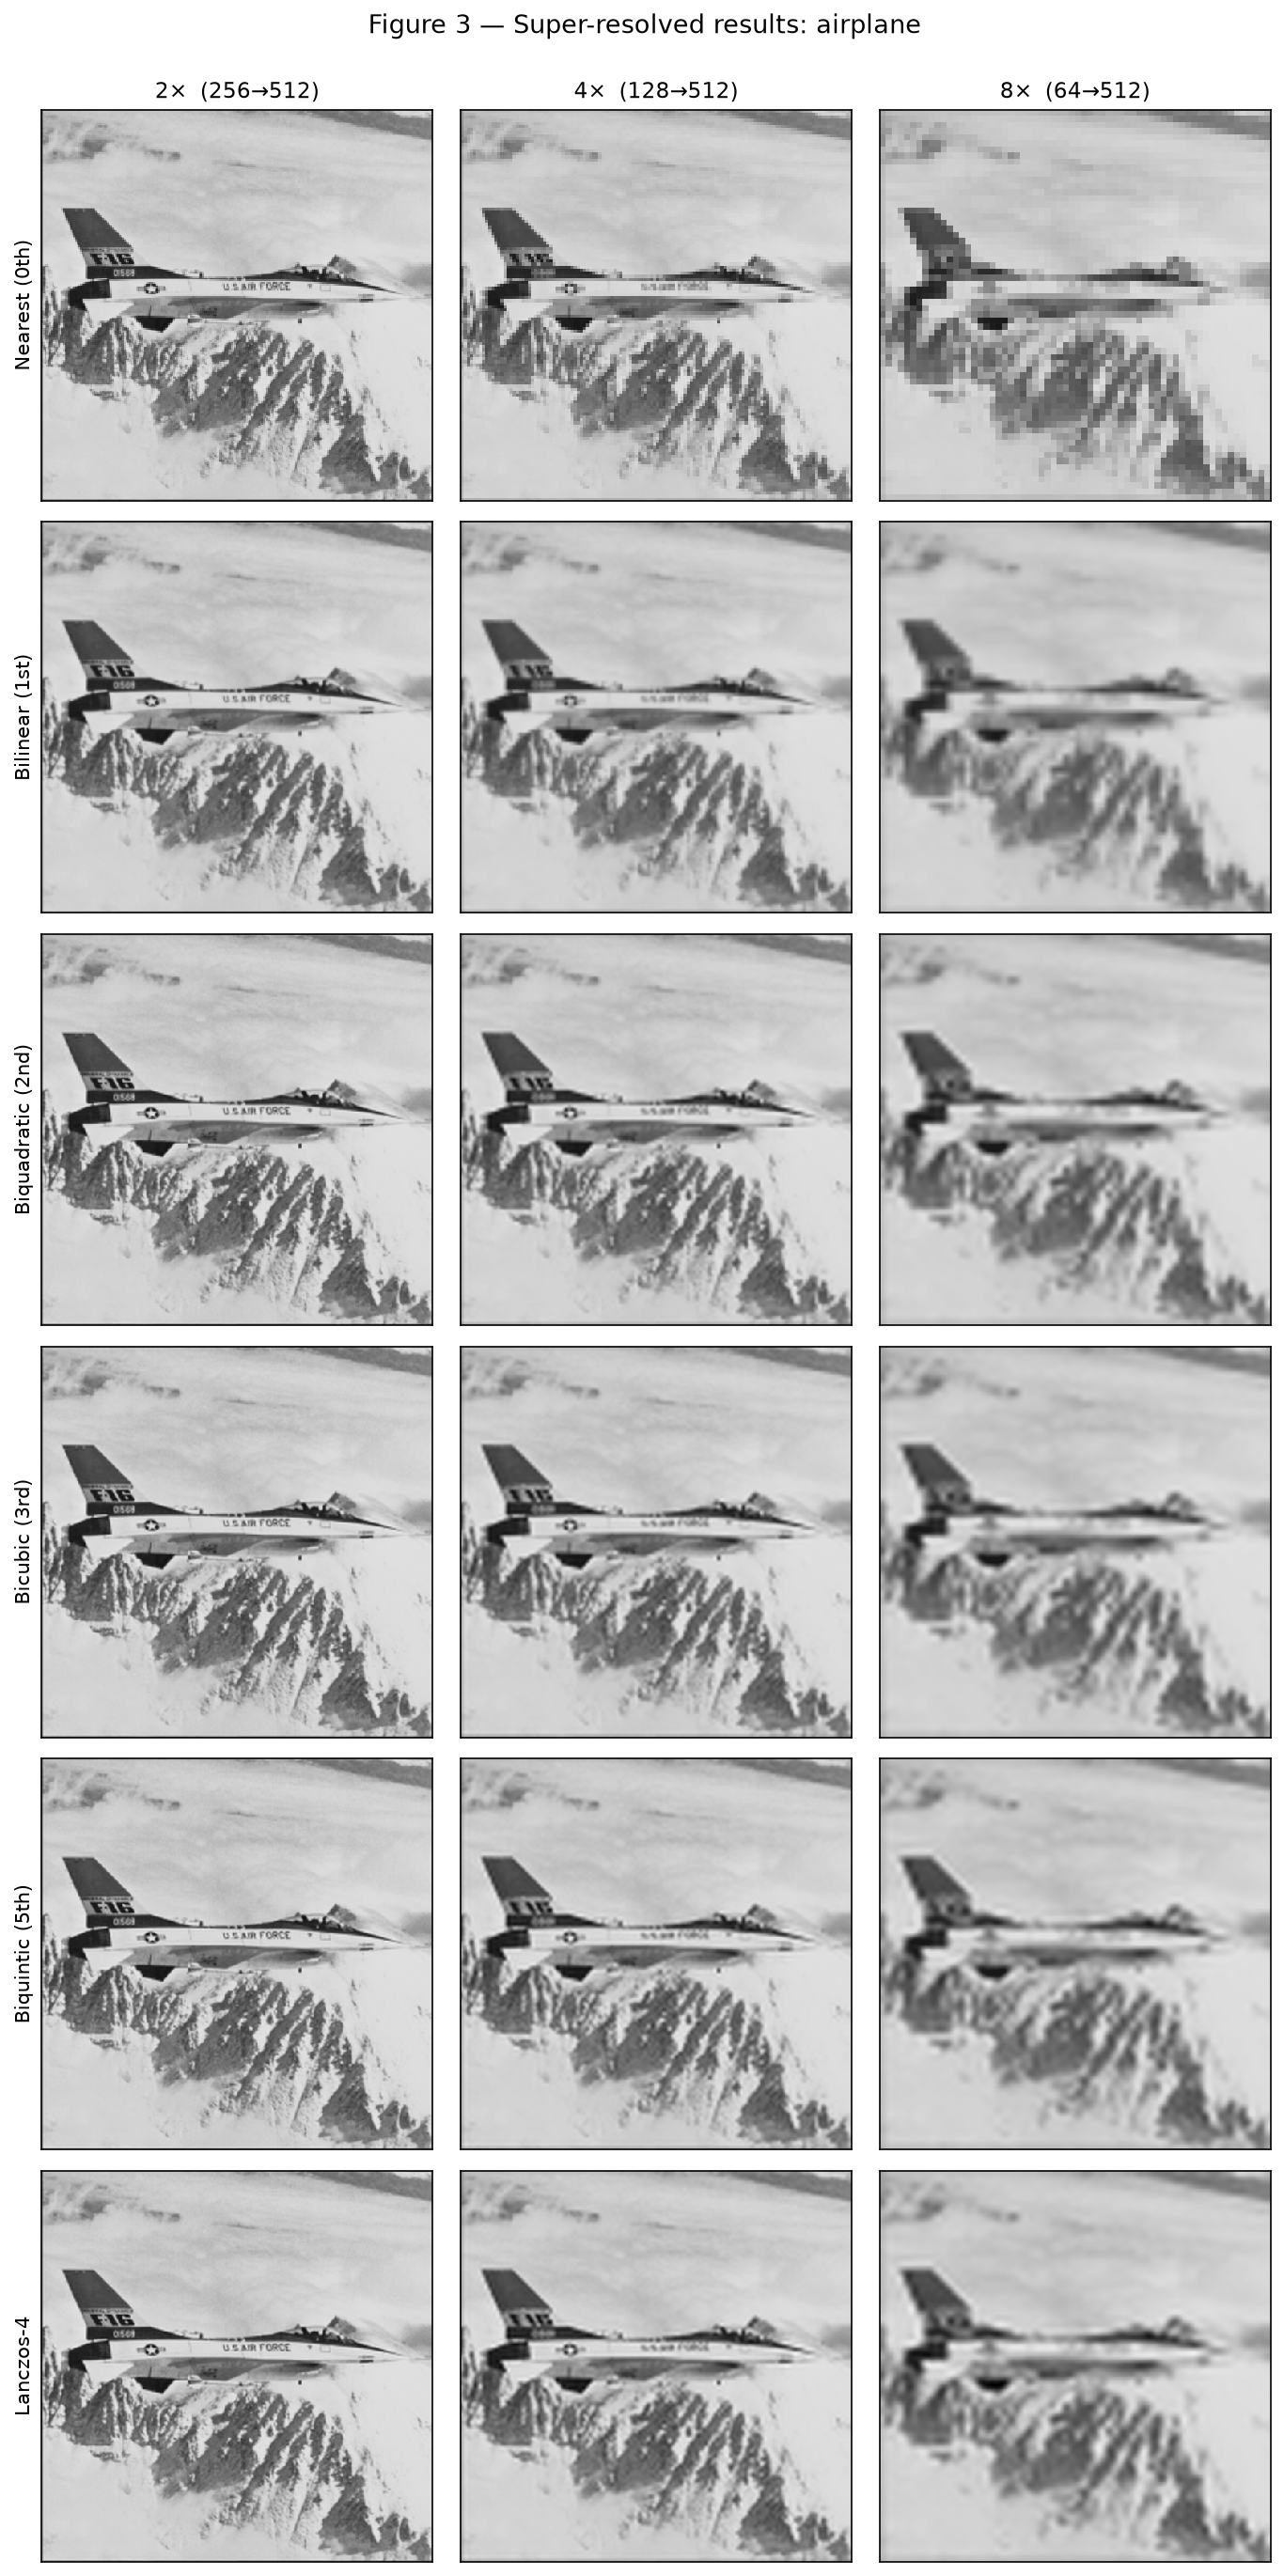
\includegraphics[height=0.86\textheight]{figures_fig3_sr_airplane.png}
\caption{Super-resolved results for \emph{airplane}: rows are interpolation methods, columns
are enlargement factors. At $2\times$ all methods except nearest neighbour are nearly
indistinguishable at this scale; at $8\times$ the gap between nearest neighbour and the rest
is large, while the differences \emph{among} the higher-order methods remain small.}
\label{fig:sr-airplane}
\end{figure}

\begin{figure}[H]
\centering
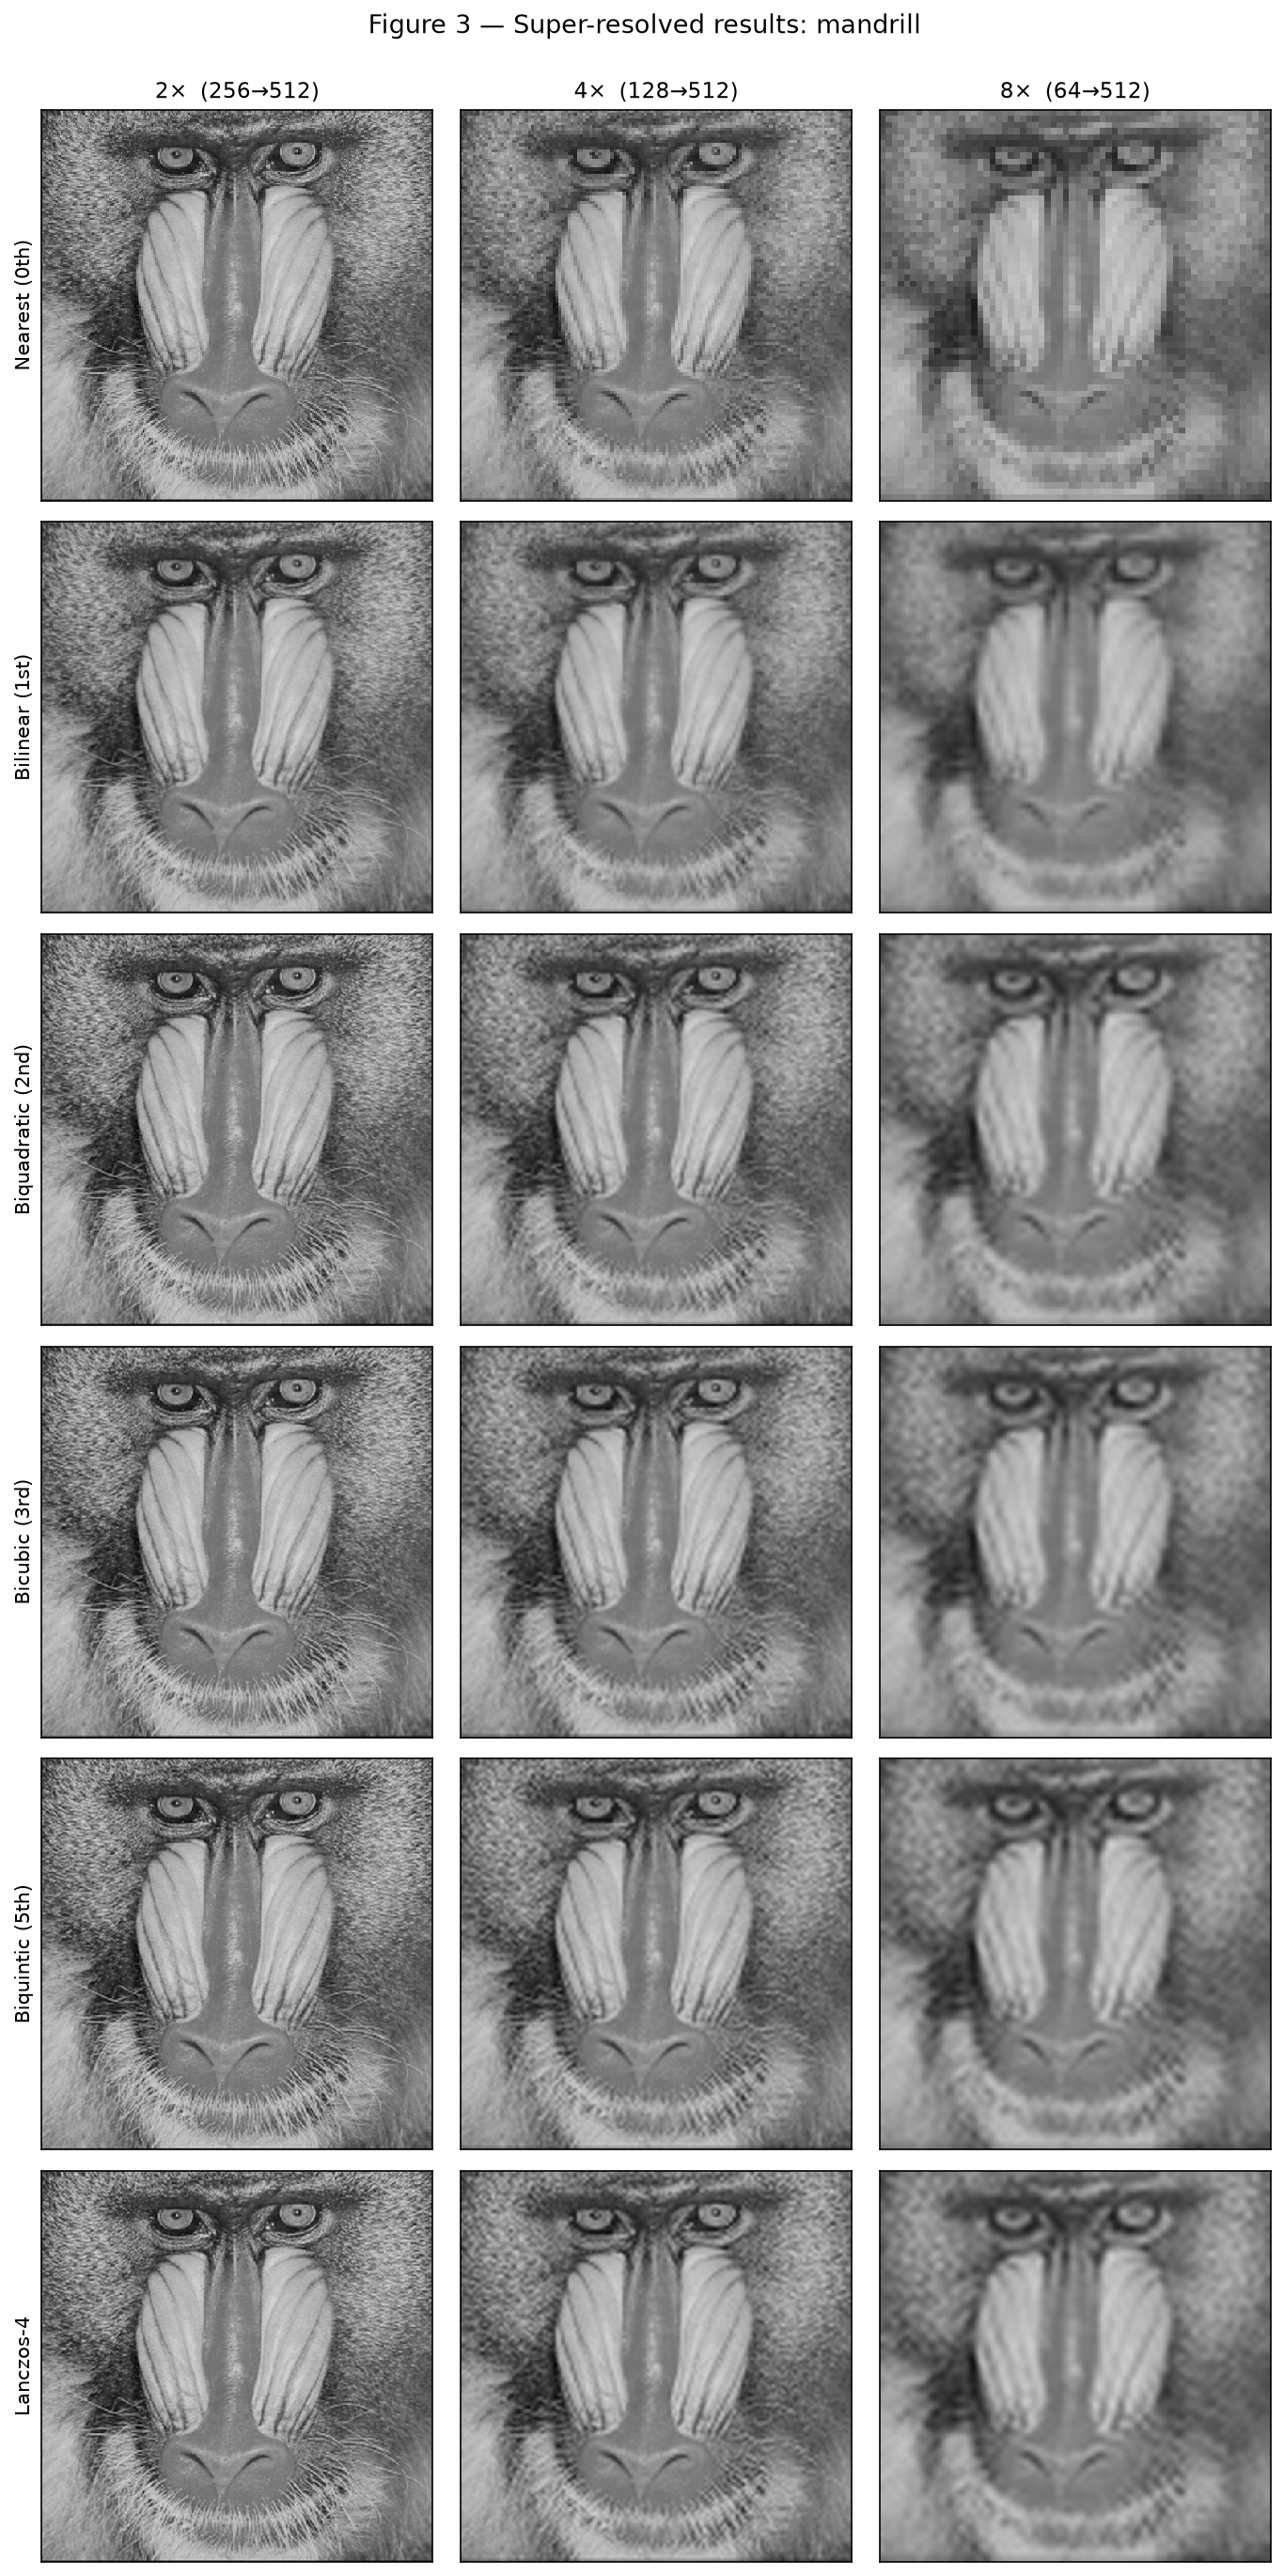
\includegraphics[height=0.86\textheight]{figures_fig3_sr_mandrill.png}
\caption{Super-resolved results for \emph{mandrill}.}
\label{fig:sr-mandrill}
\end{figure}

\begin{figure}[H]
\centering
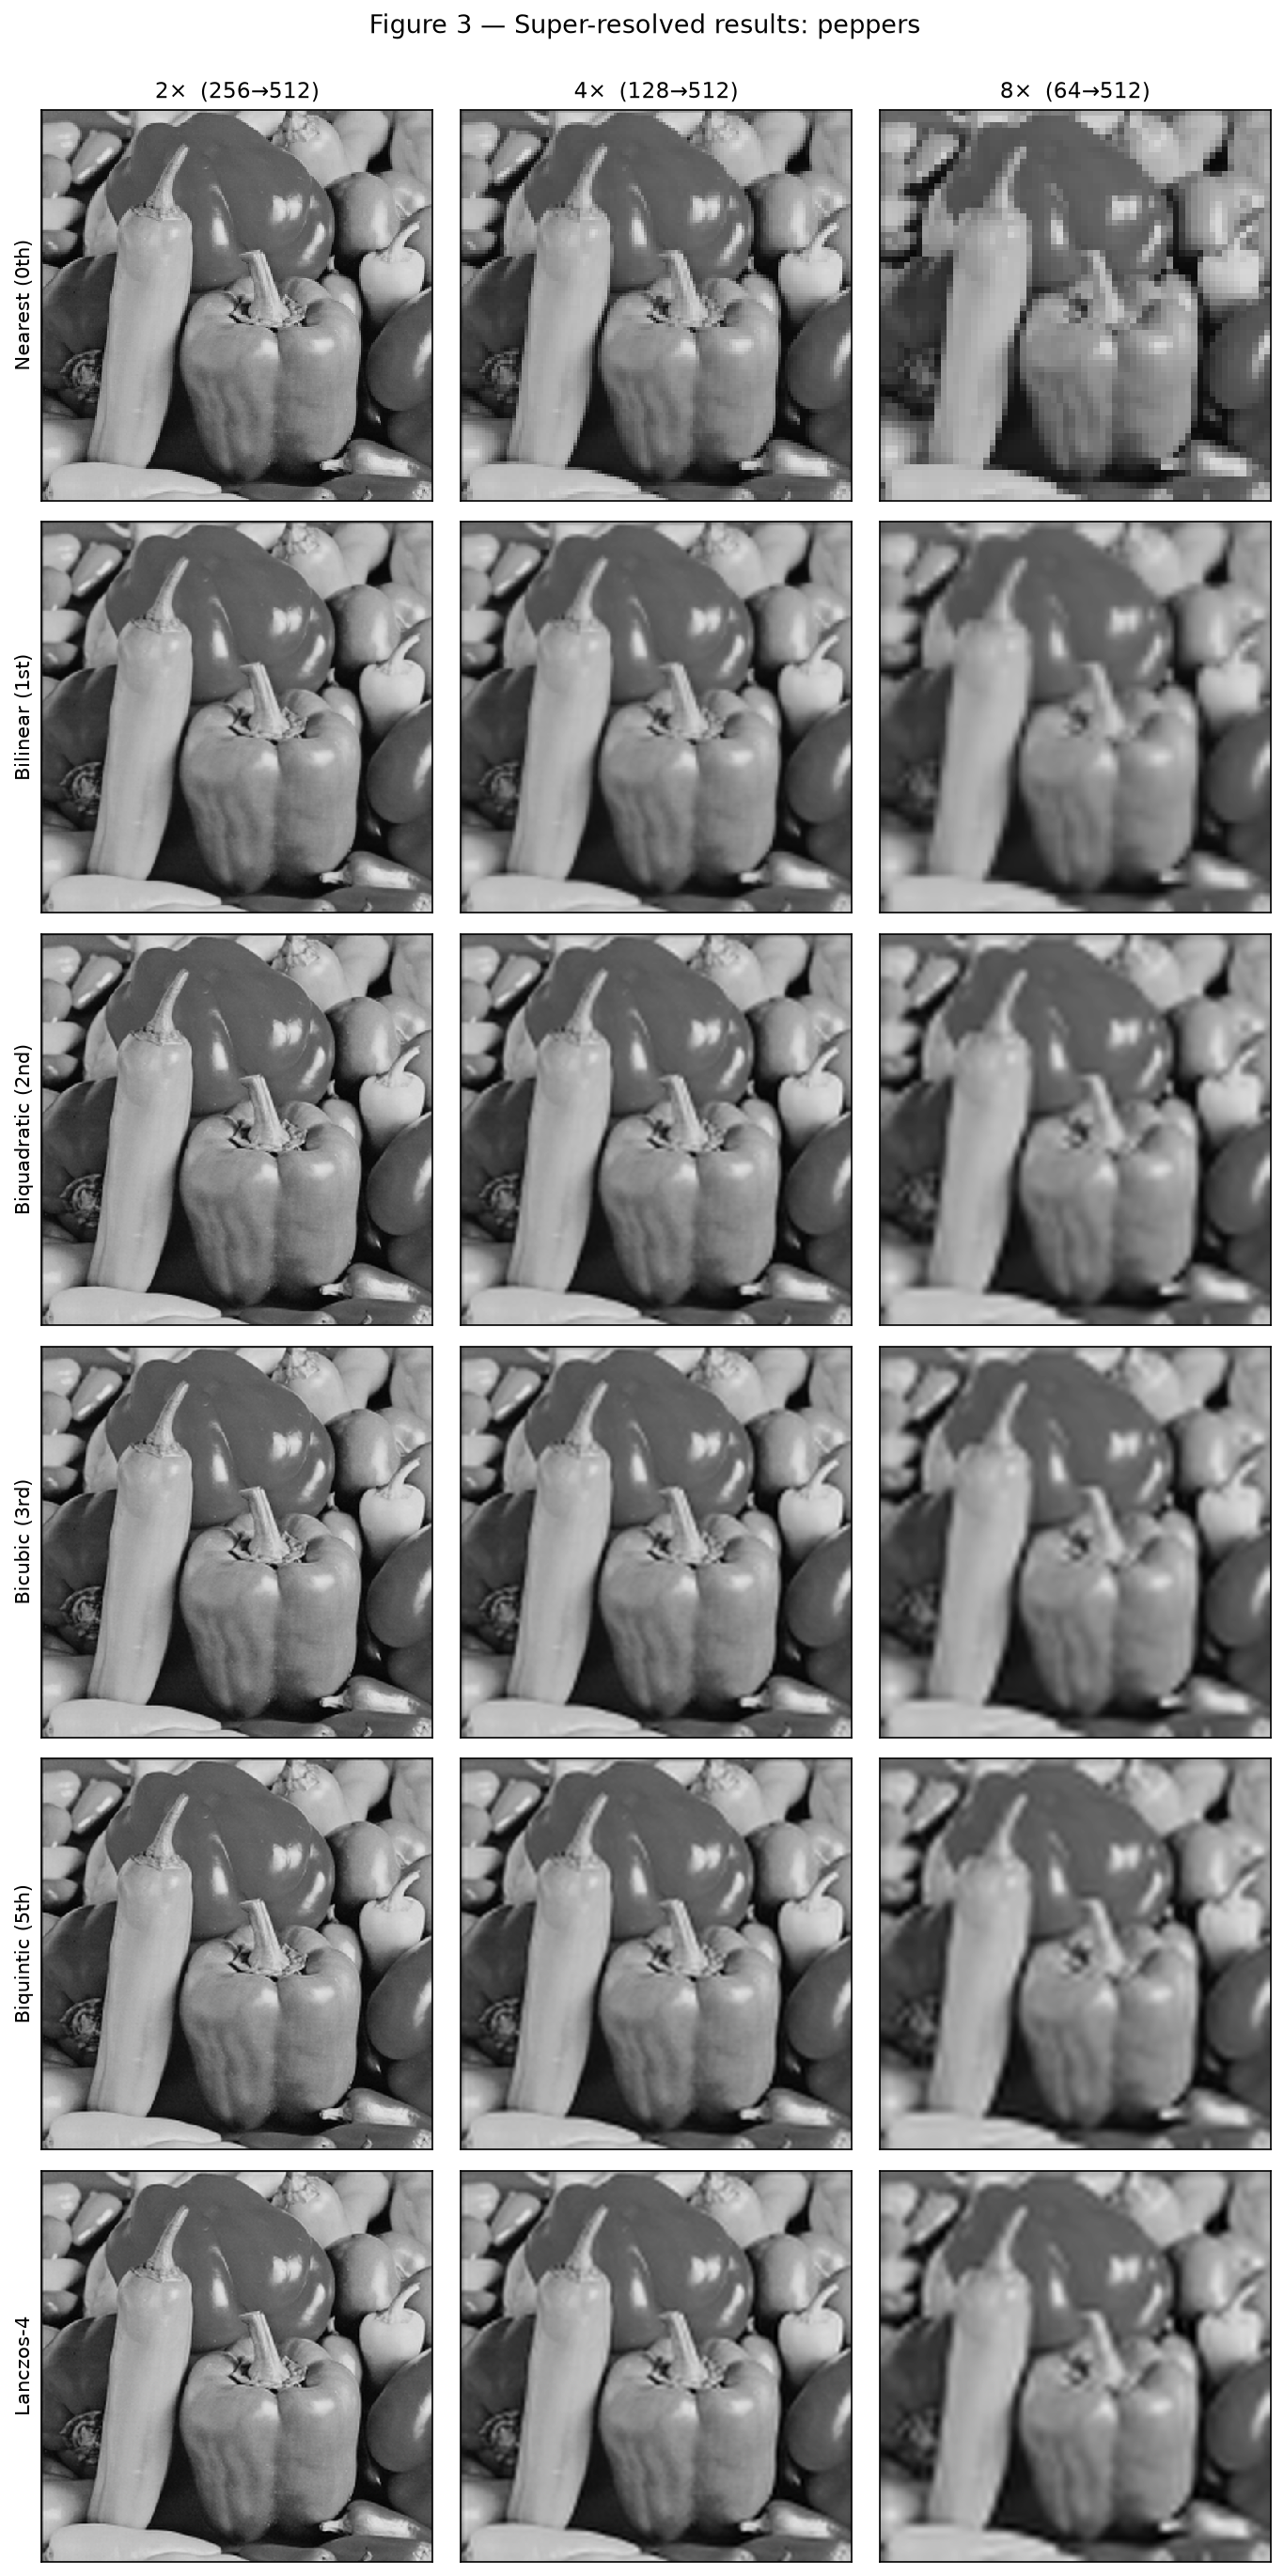
\includegraphics[height=0.86\textheight]{figures_fig3_sr_peppers.png}
\caption{Super-resolved results for \emph{peppers}.}
\label{fig:sr-peppers}
\end{figure}

\begin{figure}[H]
\centering
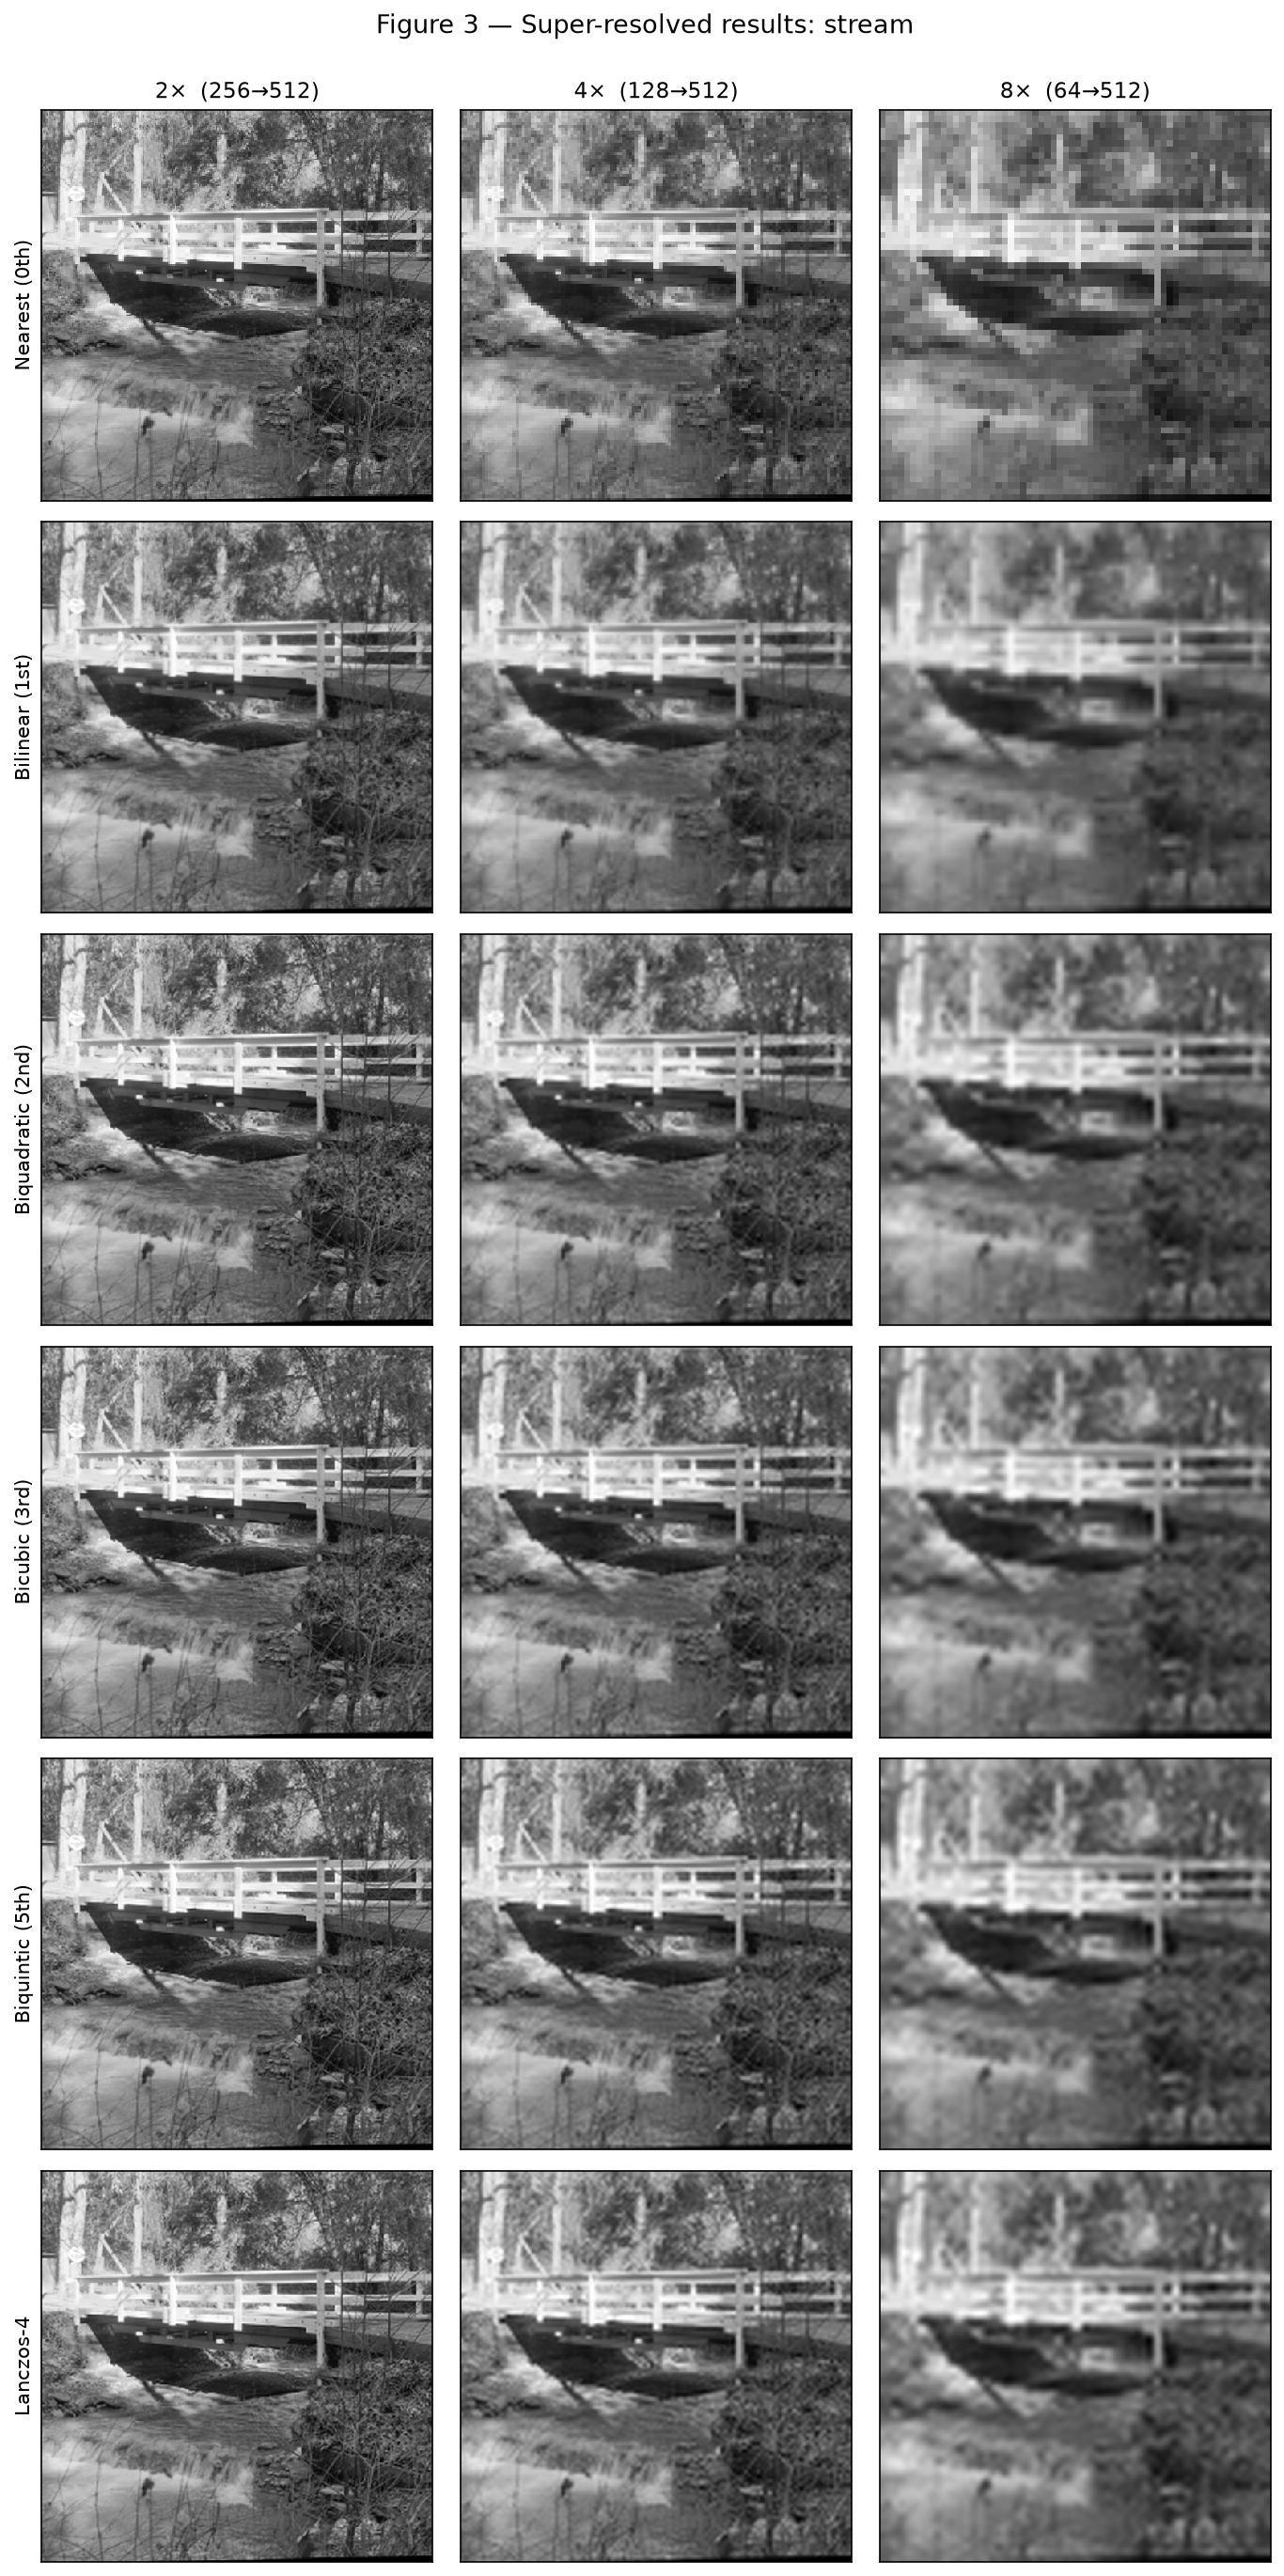
\includegraphics[height=0.86\textheight]{figures_fig3_sr_stream.png}
\caption{Super-resolved results for \emph{stream and bridge}.}
\label{fig:sr-stream}
\end{figure}

\subsection{Magnified crops}

Full-frame views cannot resolve two-pixel artefacts. The following crops are $64\times64$
regions magnified for display with nearest-neighbour screen rendering, so that what is shown
is the output of the pipeline and not a re-interpolation by the plotting library.

\begin{figure}[H]
\centering
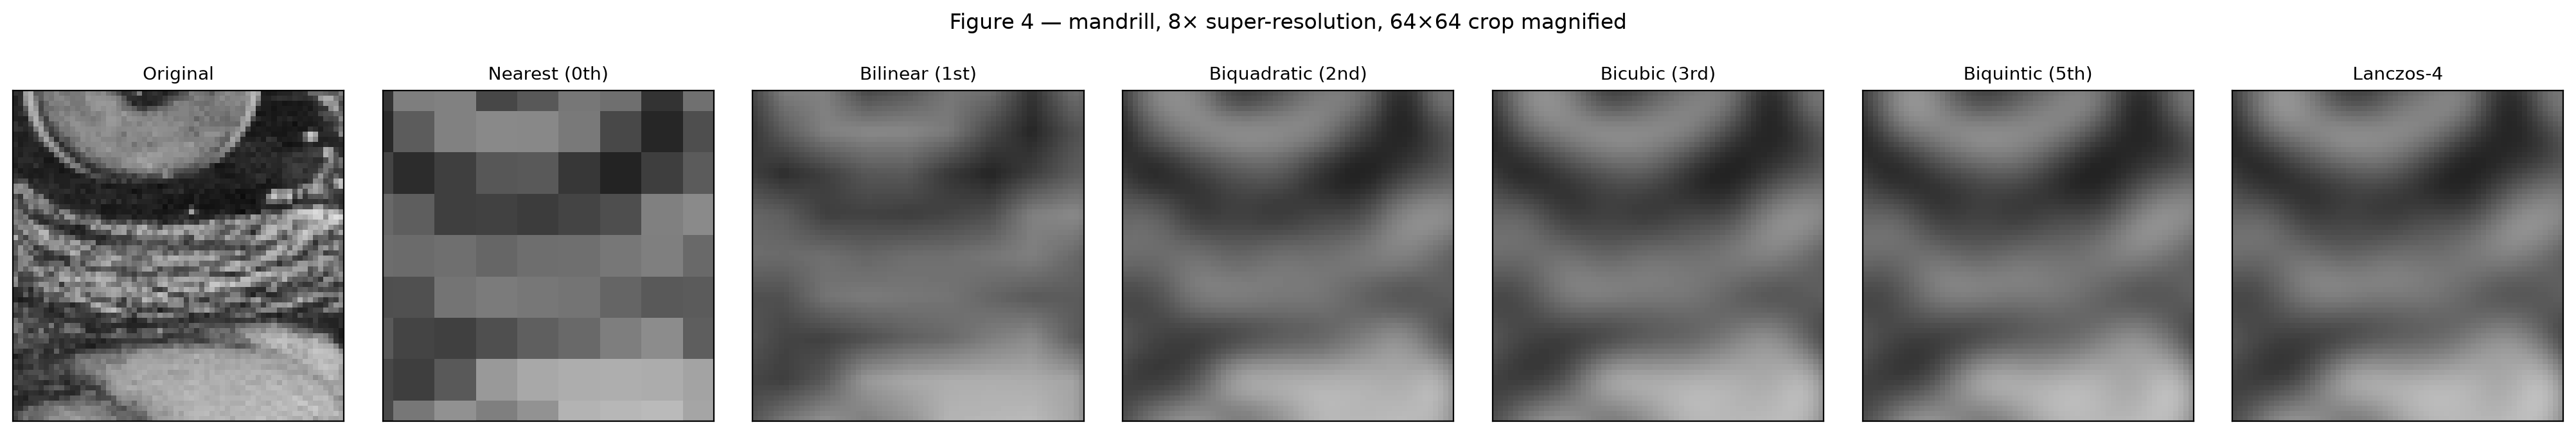
\includegraphics[width=\textwidth]{figures_fig4_crop_mandrill_8x.png}
\caption{\emph{Mandrill}, $8\times$, magnified crop. The original contains individual fur
strands and a sharp eye boundary. Nearest neighbour reproduces the input as $8\times8$
constant tiles; every higher-order method produces a smooth blob. No method recovers a single
strand --- the frequencies were destroyed during downsampling, and interpolation estimates
intensities between known samples rather than restoring lost information.}
\label{fig:crop-mandrill}
\end{figure}

\begin{figure}[H]
\centering
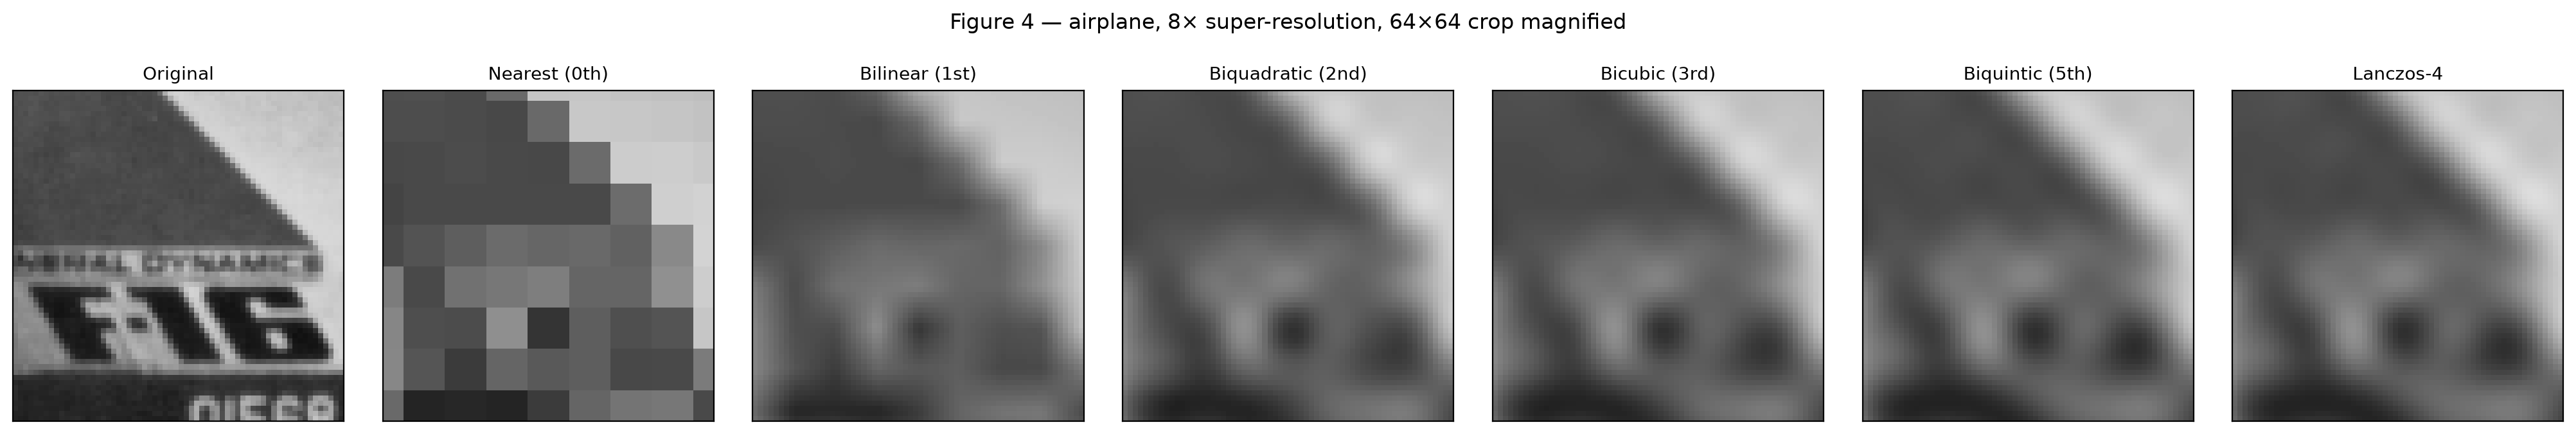
\includegraphics[width=\textwidth]{figures_fig4_crop_airplane_8x.png}
\caption{\emph{Airplane}, $8\times$, magnified crop of the tail lettering against sky. This
is the configuration in which ringing is visible: a bright/dark halo hugging the high-contrast
edge in the higher-order reconstructions, absent from nearest neighbour and bilinear.}
\label{fig:crop-airplane8}
\end{figure}

\begin{figure}[H]
\centering
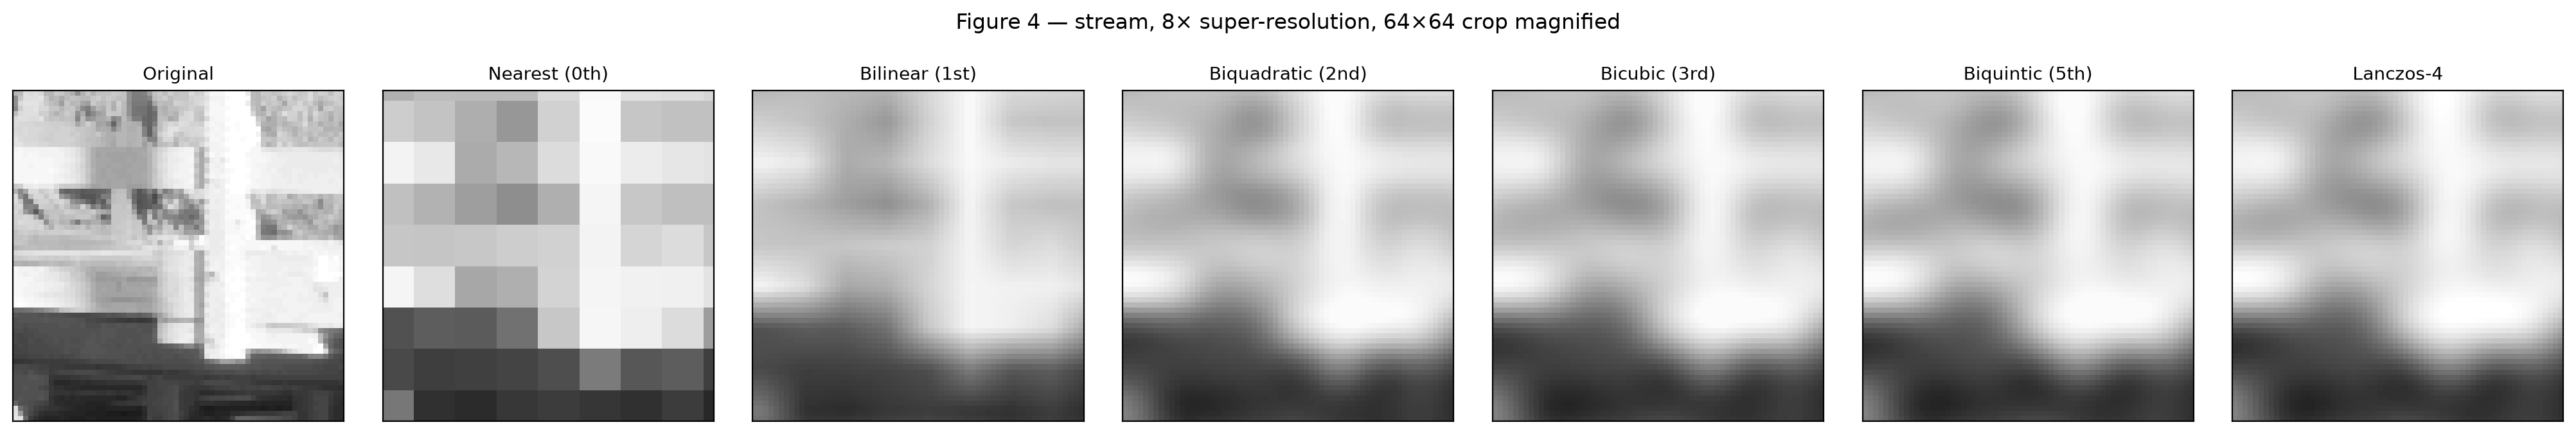
\includegraphics[width=\textwidth]{figures_fig4_crop_stream_8x.png}
\caption{\emph{Stream and bridge}, $8\times$, magnified crop of the railing against the dark
background --- staircase artefacts in nearest neighbour, halos in the higher orders.}
\label{fig:crop-stream}
\end{figure}

\begin{figure}[H]
\centering
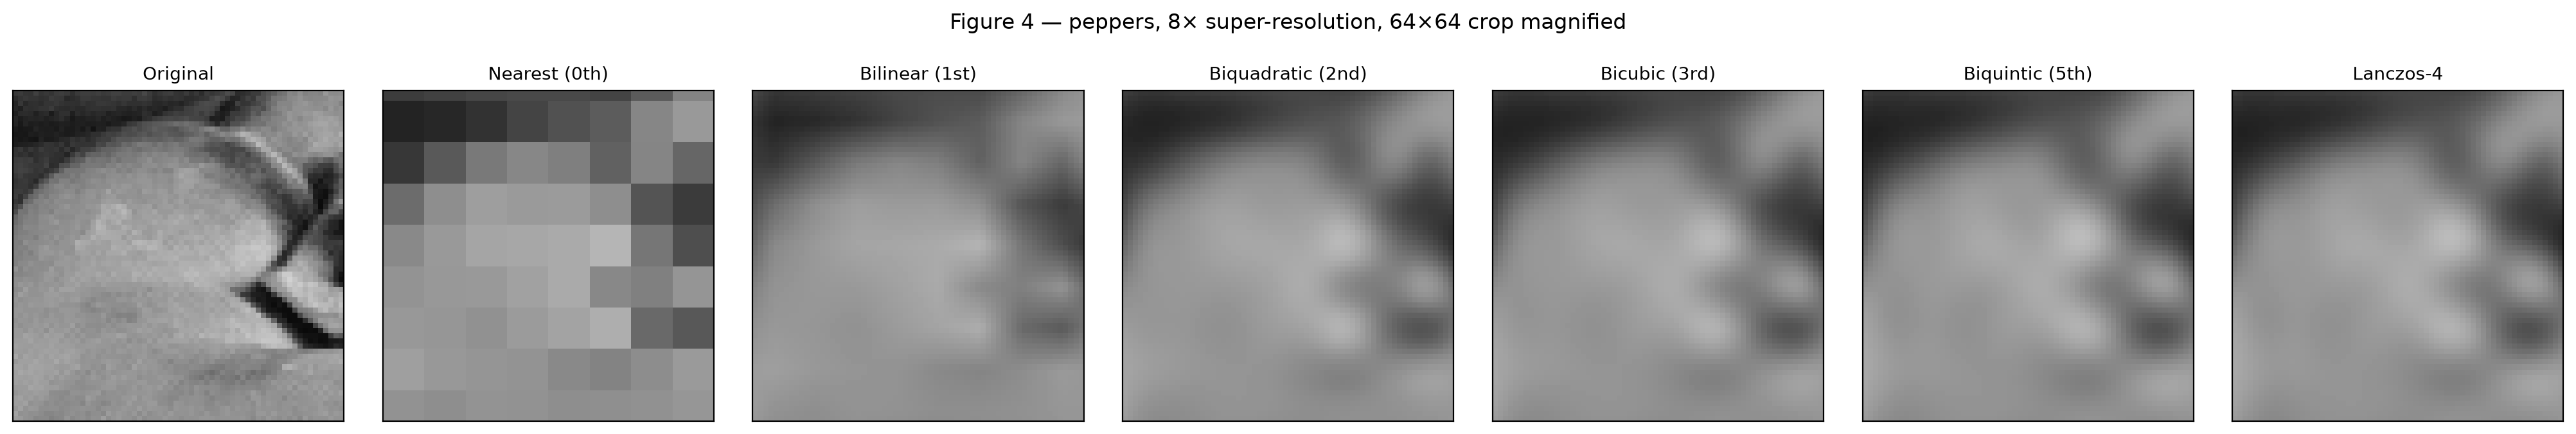
\includegraphics[width=\textwidth]{figures_fig4_crop_peppers_8x.png}
\caption{\emph{Peppers}, $8\times$, magnified crop at a bright rim against a dark pepper body.}
\label{fig:crop-peppers}
\end{figure}

%----------------------------------------------------------
\subsection{PSNR}

\begin{table}[H]
\centering
\caption{PSNR (dB) of each super-resolved image with respect to the original $512\times512$
grayscale image. Higher is better; best per column in bold.}
\label{tab:psnr}
\begin{tabular}{llccc}
\toprule
Image & Method & $2\times$ & $4\times$ & $8\times$ \\
\midrule
\multirow{6}{*}{Mandrill}
 & Nearest (0th)     & 23.35 & 20.85 & 19.70 \\
 & Bilinear (1st)    & 23.17 & 20.89 & 19.80 \\
 & Biquadratic (2nd) & \textbf{23.87} & \textbf{21.11} & \textbf{19.94} \\
 & Bicubic (3rd)     & 23.81 & 21.08 & \textbf{19.94} \\
 & Biquintic (5th)   & 23.79 & 21.07 & \textbf{19.94} \\
 & Lanczos-4         & 23.80 & 21.07 & \textbf{19.94} \\
\midrule
\multirow{6}{*}{Airplane}
 & Nearest (0th)     & 28.87 & 24.70 & 21.73 \\
 & Bilinear (1st)    & 30.11 & 25.49 & 22.22 \\
 & Biquadratic (2nd) & 31.68 & 26.38 & 22.73 \\
 & Bicubic (3rd)     & 31.77 & 26.42 & 22.73 \\
 & Biquintic (5th)   & \textbf{31.91} & \textbf{26.49} & \textbf{22.76} \\
 & Lanczos-4         & 31.90 & 26.48 & 22.75 \\
\midrule
\multirow{6}{*}{Peppers}
 & Nearest (0th)     & 29.86 & 26.01 & 22.85 \\
 & Bilinear (1st)    & 30.98 & 27.21 & 23.88 \\
 & Biquadratic (2nd) & 31.96 & 28.05 & 24.71 \\
 & Bicubic (3rd)     & 31.99 & 28.09 & 24.75 \\
 & Biquintic (5th)   & \textbf{32.04} & \textbf{28.15} & \textbf{24.81} \\
 & Lanczos-4         & \textbf{32.04} & 28.14 & \textbf{24.81} \\
\midrule
\multirow{6}{*}{Stream}
 & Nearest (0th)     & 25.68 & 22.27 & 20.28 \\
 & Bilinear (1st)    & 25.85 & 22.67 & 20.58 \\
 & Biquadratic (2nd) & \textbf{26.84} & 23.14 & \textbf{20.92} \\
 & Bicubic (3rd)     & 26.80 & 23.14 & 20.91 \\
 & Biquintic (5th)   & 26.83 & \textbf{23.16} & 20.91 \\
 & Lanczos-4         & 26.83 & \textbf{23.16} & 20.91 \\
\bottomrule
\end{tabular}
\end{table}

\subsection{SSIM}

\begin{table}[H]
\centering
\caption{SSIM of each super-resolved image with respect to the original $512\times512$
grayscale image. Higher is better; best per column in bold.}
\label{tab:ssim}
\begin{tabular}{llccc}
\toprule
Image & Method & $2\times$ & $4\times$ & $8\times$ \\
\midrule
\multirow{6}{*}{Mandrill}
 & Nearest (0th)     & 0.7546 & 0.4839 & 0.2974 \\
 & Bilinear (1st)    & 0.7006 & 0.4512 & 0.2978 \\
 & Biquadratic (2nd) & \textbf{0.7676} & 0.4940 & \textbf{0.3154} \\
 & Bicubic (3rd)     & 0.7640 & 0.4921 & 0.3143 \\
 & Biquintic (5th)   & 0.7667 & 0.4943 & 0.3150 \\
 & Lanczos-4         & 0.7669 & \textbf{0.4945} & 0.3150 \\
\midrule
\multirow{6}{*}{Airplane}
 & Nearest (0th)     & 0.9278 & 0.8042 & 0.6517 \\
 & Bilinear (1st)    & 0.9327 & 0.8191 & 0.6843 \\
 & Biquadratic (2nd) & 0.9525 & \textbf{0.8450} & \textbf{0.6990} \\
 & Bicubic (3rd)     & 0.9524 & 0.8443 & 0.6974 \\
 & Biquintic (5th)   & \textbf{0.9527} & 0.8438 & 0.6958 \\
 & Lanczos-4         & \textbf{0.9527} & 0.8438 & 0.6947 \\
\midrule
\multirow{6}{*}{Peppers}
 & Nearest (0th)     & 0.8845 & 0.7736 & 0.6133 \\
 & Bilinear (1st)    & 0.8861 & 0.8032 & 0.6906 \\
 & Biquadratic (2nd) & \textbf{0.9010} & \textbf{0.8226} & \textbf{0.7105} \\
 & Bicubic (3rd)     & 0.8998 & 0.8220 & 0.7097 \\
 & Biquintic (5th)   & 0.8990 & 0.8211 & 0.7077 \\
 & Lanczos-4         & 0.8992 & 0.8208 & 0.7068 \\
\midrule
\multirow{6}{*}{Stream}
 & Nearest (0th)     & 0.8069 & 0.5550 & 0.3329 \\
 & Bilinear (1st)    & 0.7804 & 0.5414 & 0.3457 \\
 & Biquadratic (2nd) & 0.8353 & 0.5887 & \textbf{0.3683} \\
 & Bicubic (3rd)     & 0.8338 & 0.5877 & 0.3663 \\
 & Biquintic (5th)   & 0.8363 & 0.5901 & 0.3664 \\
 & Lanczos-4         & \textbf{0.8364} & \textbf{0.5904} & 0.3664 \\
\bottomrule
\end{tabular}
\end{table}

\begin{table}[H]
\centering
\caption{PSNR and SSIM averaged over the four images. Best per column in bold.}
\label{tab:mean}
\begin{tabular}{lccc@{\hskip 1.2cm}ccc}
\toprule
& \multicolumn{3}{c}{Mean PSNR (dB)} & \multicolumn{3}{c}{Mean SSIM} \\
\cmidrule(lr){2-4}\cmidrule(lr){5-7}
Method & $2\times$ & $4\times$ & $8\times$ & $2\times$ & $4\times$ & $8\times$ \\
\midrule
Nearest (0th)     & 26.94 & 23.46 & 21.14 & 0.8435 & 0.6542 & 0.4738 \\
Bilinear (1st)    & 27.53 & 24.07 & 21.62 & 0.8250 & 0.6537 & 0.5046 \\
Biquadratic (2nd) & 28.59 & 24.67 & 22.08 & \textbf{0.8641} & \textbf{0.6876} & \textbf{0.5233} \\
Bicubic (3rd)     & 28.59 & 24.68 & 22.08 & 0.8625 & 0.6865 & 0.5219 \\
Biquintic (5th)   & \textbf{28.64} & \textbf{24.72} & \textbf{22.11} & 0.8637 & 0.6873 & 0.5212 \\
Lanczos-4         & \textbf{28.64} & 24.71 & 22.10 & 0.8638 & 0.6874 & 0.5207 \\
\bottomrule
\end{tabular}
\end{table}

\subsection{Runtime}
\label{sec:runtime}

\begin{table}[H]
\centering
\caption{Runtime in milliseconds, averaged over the four images. Each per-image value is the
mean of 10 timed runs after one warm-up call, and covers the interpolation call only.
Orders 0--5 are scikit-image; Lanczos-4 is OpenCV.}
\label{tab:runtime}
\begin{tabular}{lccc}
\toprule
Method & $2\times$ ($256\!\to\!512$) & $4\times$ ($128\!\to\!512$) & $8\times$ ($64\!\to\!512$) \\
\midrule
Nearest (0th)     &  1.108 &  1.028 &  1.023 \\
Bilinear (1st)    &  2.665 &  2.430 &  2.474 \\
Biquadratic (2nd) &  5.221 &  4.584 &  4.231 \\
Bicubic (3rd)     &  7.621 &  6.755 &  6.724 \\
Biquintic (5th)   & 16.002 & 14.646 & 14.360 \\
\midrule
Lanczos-4$^{\dagger}$ & 0.215 & 0.166 & 0.139 \\
\bottomrule
\multicolumn{4}{l}{\footnotesize $^{\dagger}$ Different library --- see discussion in
Section~\ref{sec:disc-runtime}.}
\end{tabular}
\end{table}

\begin{table}[H]
\centering
\caption{Quality versus cost, averaged over all four images and all three enlargement
factors.}
\label{tab:summary}
\begin{tabular}{lccc}
\toprule
Method & Mean PSNR (dB) & Mean SSIM & Mean runtime (ms) \\
\midrule
Nearest (0th)     & 23.85 & 0.6572 &  1.053 \\
Bilinear (1st)    & 24.40 & 0.6611 &  2.523 \\
Biquadratic (2nd) & 25.11 & \textbf{0.6917} &  4.679 \\
Bicubic (3rd)     & 25.12 & 0.6903 &  7.033 \\
Biquintic (5th)   & \textbf{25.16} & 0.6907 & 15.003 \\
Lanczos-4         & 25.15 & 0.6906 &  0.173 \\
\bottomrule
\end{tabular}
\end{table}

%==========================================================
\section{Discussion}

\subsection{Quality across enlargement factors}

Quality falls monotonically from $2\times$ to $4\times$ to $8\times$ for every method on
every image, without a single exception across all 24 method--image combinations. Averaged
over the four images, bicubic drops from 28.59\,dB at $2\times$ to 24.68\,dB at $4\times$ and
22.08\,dB at $8\times$ --- roughly 3.9\,dB for the first step and a further 2.6\,dB for the
second. SSIM degrades more steeply in relative terms, from 0.86 to 0.69 to 0.52.

The reason is straightforward. At $2\times$, one in four output pixels corresponds to a
retained sample; at $8\times$ only one in sixty-four does, so $63/64$ of the output is
estimated. More importantly, the area-averaging stage acts as a low-pass filter whose cutoff
scales with the decimation factor, and the high-frequency content it removes is not present in
any form in the low-resolution image. Interpolation reconstructs intensities \emph{between}
known samples; it does not invert a low-pass filter. Figure~\ref{fig:crop-mandrill} makes this
concrete: the fur strands visible in the original are absent from all six $8\times$
reconstructions.

\subsection{Visual differences among the methods}

Nearest neighbour is visibly distinct from everything else. It replicates each input sample
over an $s \times s$ block, producing hard tile boundaries that are obvious at $8\times$
(Figure~\ref{fig:sr-airplane}, top row) and still detectable as jagged diagonal edges at
$2\times$.

Bilinear removes the blocking but at the cost of noticeable blur, since every interpolated
pixel is a weighted average of its neighbours. The gain from nearest to bilinear is
0.59\,dB at $2\times$ and 0.48\,dB at $8\times$ on average.

Beyond first order the methods converge sharply. Biquadratic, bicubic, biquintic and Lanczos-4
differ by at most 0.06\,dB in the averaged results at any factor, and are visually almost
indistinguishable in Figures~\ref{fig:sr-airplane}--\ref{fig:sr-stream}. The step from first
to second order is worth about 1.06\,dB; the step from second to fifth order is worth
0.05\,dB. Higher kernel order is therefore not monotonically better in any practically
meaningful sense past the third order, and on SSIM the ordering actually reverses ---
biquadratic attains the best mean SSIM at all three factors, ahead of bicubic and biquintic.

\subsection{Artefacts}

\textbf{Blocking and staircase.} Confined to nearest neighbour, and worsening with the
enlargement factor. Figure~\ref{fig:crop-mandrill} shows the $8\times8$ constant tiles
directly. This is the expected consequence of a zeroth-order kernel, which models intensity as
constant over the region a pixel represents.

\textbf{Blur.} Present in all interpolated results and dominant at $8\times$. It is most
damaging on textured content, where it is the principal reason the mandrill scores so poorly.

\textbf{Ringing and overshoot.} Restricted to the kernels of order $\ge 2$, whose impulse
responses have negative lobes. Near a high-contrast edge these lobes drive the reconstruction
beyond the range of the surrounding samples, producing a bright band on the light side and a
dark band on the dark side. This is visible in Figure~\ref{fig:crop-airplane8} at the tail
lettering and in Figure~\ref{fig:crop-stream} at the railing. Nearest neighbour and bilinear
have non-negative kernels and cannot overshoot: their outputs are bounded by the convex hull
of the input samples. All results reported here were clipped to $[0,255]$ before evaluation,
which suppresses the most extreme excursions but does not remove the halo itself.

\subsection{Reconstruction quality versus runtime}
\label{sec:disc-runtime}

Within the scikit-image family the cost scales with the kernel support, as expected: nearest
neighbour at roughly 1.0\,ms, bilinear at 2.5\,ms, biquadratic at 4.7\,ms, bicubic at 7.0\,ms
and biquintic at 15.0\,ms on average. The quality returns do not scale similarly. Moving from
nearest to bilinear costs $2.4\times$ the runtime for 0.55\,dB; from bilinear to biquadratic
costs a further $1.9\times$ for 0.71\,dB; from biquadratic to biquintic costs $3.2\times$ for
0.05\,dB. The knee of the curve sits at second or third order, which is consistent with
bicubic being the conventional default in practice.

The Lanczos-4 figure requires care. At 0.173\,ms average it is roughly $87\times$ faster than
biquintic while matching it in quality, but this is not a statement about kernel cost --- a
windowed-sinc kernel does more arithmetic per output pixel, not less. It reflects the
implementation: OpenCV uses hand-optimised fixed-point SIMD C++, whereas scikit-image performs
\texttt{float64} spline pre-filtering followed by evaluation through a more general code path.
The correct conclusion is that implementation quality dominates kernel order as a determinant
of wall-clock cost at these image sizes, and that runtime comparisons across libraries should
not be read as algorithmic comparisons.

It is also worth noting that runtime is essentially independent of image content --- the
spread across the four images at a fixed method and factor is small and attributable to
measurement noise --- and that it varies only weakly with the enlargement factor, since the
output size is fixed at $512\times512$ and the work is dominated by the number of output
pixels rather than the number of input samples.

\subsection{Dependence on image content}

The results depend strongly on content, in two separate ways.

\textbf{Absolute quality.} At $8\times$, peppers reaches 24.81\,dB while mandrill reaches only
19.94\,dB --- a gap of almost 5\,dB between the smoothest and the most textured image, under
identical processing. Smooth regions are well approximated by low-order polynomials, which is
precisely the assumption every one of these kernels encodes. Dense texture violates it.

\textbf{Spread between methods.} The gap between the best and worst method is widest on
edge-dominated content and narrowest on texture. On airplane at $2\times$ the spread is
3.04\,dB (28.87 to 31.91); on mandrill at $8\times$ it is 0.24\,dB (19.70 to 19.94). Where
the signal has been destroyed, the choice of interpolator ceases to matter --- all six methods
are reconstructing from the same impoverished data and converge to nearly the same answer. In
flat regions the methods also agree, for the opposite reason: every interpolator returns
approximately the local mean. It is only at edges, where a genuine decision about the
intensity profile must be made, that the kernels separate.

\subsection{A case where nearest neighbour wins}

One result initially appears anomalous and is worth stating explicitly. On mandrill at
$2\times$, nearest neighbour outperforms bilinear on both metrics: 23.35\,dB versus 23.17\,dB
on PSNR, and 0.7546 versus 0.7006 on SSIM. The same inversion appears in the SSIM averages,
where nearest neighbour beats bilinear at $2\times$ (0.8435 versus 0.8250) and ties it at
$4\times$.

This is not an error. At $2\times$, nearest neighbour reproduces every retained sample exactly
and preserves local contrast, adding only blocking. Bilinear replaces interpolated pixels with
weighted averages, which reduces local variance everywhere. On an image whose content is
almost entirely high-frequency texture, the variance loss costs more than the blocking does.
SSIM penalises this more sharply than PSNR because its contrast and structure terms respond
directly to local variance, whereas PSNR sees only squared error. The practical implication is
that PSNR and SSIM do not always rank methods identically, and that the usual assumption
``higher order is better'' presumes locally smooth content.

%==========================================================
\section{Conclusion}

Across four images, three enlargement factors and six interpolation methods, the results
support four conclusions. Reconstruction quality degrades monotonically with the enlargement
factor and cannot recover frequencies removed during downsampling. The largest quality gain
comes from moving off zeroth order; gains beyond second or third order are negligible while
costs continue to grow. Each kernel family has a characteristic artefact --- blocking for
zeroth order, blur for first order, ringing for orders two and above --- and the choice among
them is a trade between these rather than a strict ordering. Finally, all of these effects
are modulated by image content: on smooth images every method performs well and similarly, on
edge-dominated images the method choice matters most, and on heavily textured images at high
enlargement factors no interpolation method performs well at all.

%==========================================================
\section*{Reproducibility}

All results were generated by the accompanying Python notebook. Per-configuration numbers are
written to \texttt{results/metrics.csv} (72 rows); every table in this report is derived from
that file. The pipeline contains no stochastic component and reproduces bit-identically on
re-run. Libraries used: NumPy, OpenCV, scikit-image, SciPy, pandas, Matplotlib.

\end{document}